% radiosynth - From MHD to MHz: thermal gyroresonance emission, equations and implementation
% Copyright (C) 2026 Soumitra Hazra
% Compile with: pdflatex radiosynth_gyroresonance.tex (twice)
\documentclass[11pt,a4paper]{article}
\usepackage[T1]{fontenc}
\usepackage{lmodern}
\usepackage[margin=2.4cm]{geometry}
\usepackage{amsmath,amssymb,bm}
\usepackage{booktabs,array,longtable}
\usepackage{graphicx}
\usepackage{xcolor}
\usepackage{tikz}
\usetikzlibrary{arrows.meta,decorations.pathreplacing,calc}
\usepackage{enumitem}
\usepackage[font=small,labelfont=bf]{caption}
\usepackage[colorlinks=true,linkcolor=blue!50!black,citecolor=blue!50!black,urlcolor=blue!50!black]{hyperref}

\definecolor{accent}{RGB}{31,78,121}
\newcommand{\code}[1]{\texttt{#1}}
\newcommand{\vect}[1]{\bm{#1}}
\newcommand{\dd}{\mathrm{d}}
\newcommand{\kB}{k_\mathrm{B}}
\newcommand{\ncr}{n_\mathrm{cr}}
\newcommand{\nuB}{\nu_B}
\newcommand{\rsun}{R_\odot}
\setlist{itemsep=2pt,topsep=4pt}
\setlength{\parskip}{3pt}
\setlength{\emergencystretch}{2.5em}

\newenvironment{incode}{\par\smallskip\noindent\begin{minipage}{\linewidth}\small\color{accent!80!black}\textbf{In the code.}~}{\end{minipage}\par\smallskip}

\hypersetup{pdftitle={Thermal gyroresonance emission in radiosynth},pdfauthor={Soumitra Hazra}}

\begin{document}

\begin{center}
{\LARGE\bfseries\color{accent} Thermal gyroresonance emission in \textsf{radiosynth}\par}
\vspace{0.3cm}
{\large Equations, derivation and numerical implementation\par}
\vspace{0.4cm}
{\normalsize Soumitra Hazra\par}
\vspace{0.1cm}
{\small \textsf{radiosynth} 2.2.0 --- \emph{From MHD to MHz} --- November 2026\par}
{\small \url{https://github.com/soumitrahazra/radiosynth}\par}
\end{center}

\begin{abstract}
\noindent This note collects every equation used by \textsf{radiosynth} to compute the
thermal gyroresonance (GR) emission of a magnetohydrodynamic (MHD) model, together with the
magnetised free--free emission that accompanies it, in Stokes $I$ and $V$. It starts from the
cold-plasma magneto-ionic modes, derives the optical depth of a harmonic layer from the
low-temperature expansion of the gyromagnetic absorption coefficient, and then describes how
the code finds the layers along straight lines of sight, how it solves the polarised
radiative transfer for the two circular polarisations (or the two modes), and how it turns
the result into brightness temperatures, polarisation and fluxes. Each section ends with the
corresponding function of the code (\code{radiosynth/gyroresonance/}, \code{common/magnetoionic.py},
\code{bremsstrahlung/magnetized.py}), so that the equations can be checked line by line.
\end{abstract}

\tableofcontents

%======================================================================
\section{Overview}
%======================================================================

A thermal electron gyrating in a magnetic field $B$ radiates and absorbs at the harmonics
$s\nuB$ of its gyrofrequency $\nuB=eB/(2\pi m_e)$. In a Maxwellian plasma with
$\kB T_e\ll m_ec^2$ the absorption at a given observing frequency $\nu$ is therefore confined
to thin \emph{harmonic layers}, the surfaces on which
\begin{equation}
  \nu = s\,\nuB(\vect r), \qquad s=1,2,3,\ldots
  \label{eq:resonance}
\end{equation}
Over active regions, where $B$ reaches several hundred to a few thousand gauss, the
layers with $s=2$ and $s=3$ are usually optically thick at 1--20\,GHz, so the brightness
temperature of the radio source equals the coronal electron temperature at the height of the
layer. Gyroresonance emission is the main microwave signature of sunspots, and its circular
polarisation measures the coronal magnetic field.

\textsf{radiosynth} computes this emission in five steps (Fig.~\ref{fig:scheme}):
\begin{enumerate}
  \item set up the image plane and one straight line of sight per pixel, and sample
        $n_e$, $T_e$ and $\vect B$ of the model at equally spaced nodes along it
        (Sect.~\ref{sec:geometry});
  \item evaluate the magneto-ionic parameters and the mode polarisations
        (Sect.~\ref{sec:modes});
  \item compute the magnetised free--free optical depth of every step
        (Sect.~\ref{sec:ff}) and the optical depth of every harmonic layer crossed in the
        step (Sects.~\ref{sec:opacity}--\ref{sec:layers});
  \item solve the radiative transfer for the two polarisations
        (Sects.~\ref{sec:kirchhoff}, \ref{sec:transfer} and \ref{sec:coupling});
  \item convert to Stokes $I$, $V$, brightness temperatures and fluxes, and compute the
        diagnostics (Sects.~\ref{sec:output} and \ref{sec:diag}).
\end{enumerate}
Refraction is negligible where gyroresonance emission forms ($\nu\gg\nu_p$), so the rays
are straight; the refractive ray tracer of \textsf{radiosynth} is used only for the
free--free and simplistic mechanisms.

\begin{figure}[t]
\centering
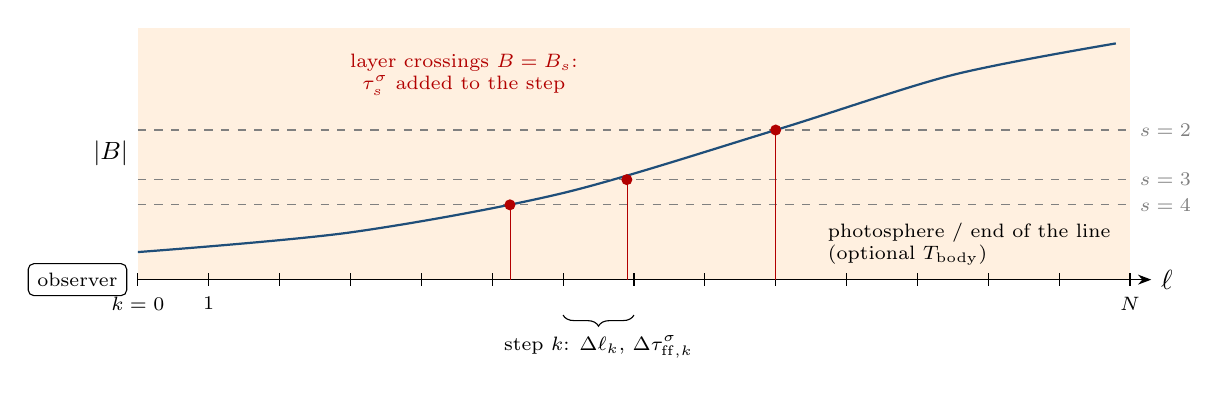
\begin{tikzpicture}[x=0.9cm,y=1cm,>=Stealth]
  % field strength profile
  \fill[orange!12] (0,0) rectangle (14,3.2);
  \draw[->] (0,0) -- (14.3,0) node[right]{$\ell$};
  \node[left] at (0,1.6) {\small $|B|$};
  \draw[thick,accent] plot[smooth] coordinates {(0,0.35) (3,0.6) (6,1.1) (9,1.9) (11.5,2.6) (13.8,3.0)};
  % observer
  \node[draw,fill=white,rounded corners=2pt,font=\scriptsize,anchor=east] at (-0.15,0.0) {observer};
  % harmonic levels
  \foreach \y/\s in {0.95/4, 1.27/3, 1.9/2} {
     \draw[gray,dashed] (0,\y) -- (14,\y);
     \node[gray,right,font=\scriptsize] at (14,\y) {$s=\s$};
  }
  % nodes
  \foreach \x in {0,1,...,14} { \draw (\x,-0.08) -- (\x,0.08); }
  \node[below,font=\scriptsize] at (0,-0.1) {$k=0$};
  \node[below,font=\scriptsize] at (1,-0.1) {$1$};
  \node[below,font=\scriptsize] at (14,-0.1) {$N$};
  % crossings
  \foreach \x/\y in {5.25/0.95, 6.9/1.27, 9.0/1.9} {
     \fill[red!70!black] (\x,\y) circle (2pt);
     \draw[red!70!black,very thin] (\x,\y) -- (\x,0);
  }
  \node[red!70!black,font=\scriptsize,align=center] at (4.6,2.6) {layer crossings $B=B_s$:\\ $\tau_s^\sigma$ added to the step};
  \draw[decorate,decoration={brace,mirror,amplitude=4pt}] (6,-0.45) -- (7,-0.45)
       node[midway,below=4pt,font=\scriptsize]{step $k$: $\Delta\ell_k$, $\Delta\tau^\sigma_{\mathrm{ff},k}$};
  \node[font=\scriptsize,align=left,anchor=west] at (9.6,0.45) {photosphere / end of the line\\ (optional $T_\mathrm{body}$)};
\end{tikzpicture}
\caption{How a line of sight is treated. The model is sampled at nodes $k=0\ldots N$, from
the observer inwards. Each step carries the free--free optical depth of its mid-point, plus the
optical depth of every harmonic layer $\nu=s\nuB$ whose field strength lies between the
field strengths of its two nodes. The layers are much thinner than a step and are treated as
discontinuities.}
\label{fig:scheme}
\end{figure}

%======================================================================
\section{Notation, units and constants}\label{sec:notation}
%======================================================================

The code works in SI units, with the magnetic field in gauss and lengths of the model in
coordinate units (solar or stellar radii) converted to metres with the grid's
\code{length\_unit}. In SI, $e^2$ is replaced by $e^2/4\pi\varepsilon_0$ in every Gaussian
formula below. The main quantities are:

\begin{center}
\small
\begin{longtable}{@{}l p{8.3cm} l@{}}
\toprule
Symbol & Meaning & Value / unit \\
\midrule
$\nu$ & observing frequency & Hz \\
$n_e,\ T_e$ & electron density, electron temperature & m$^{-3}$, K \\
$\vect B,\ B=|\vect B|$ & magnetic field and its strength & G \\
$\hat{\vect k}$ & unit vector along the line of sight, \emph{towards the observer} & --- \\
$\theta$ & angle between $\vect B$ and $\hat{\vect k}$, $\cos\theta=\vect B\cdot\hat{\vect k}/B$ & --- \\
$\nuB$ & electron gyrofrequency, $eB/(2\pi m_e)$ & $2.799249$\,MHz\,G$^{-1}\times B$ \\
$\nu_p$ & plasma frequency, $\nu_p^2=e^2n_e/(4\pi^2\varepsilon_0 m_e)$ & Hz \\
$\ncr$ & critical density, $\ncr=\pi m_e\nu^2/(e^2/4\pi\varepsilon_0)$ & $1.2404\times10^{16}$\,m$^{-3}$ at 1\,GHz \\
$X$ & $(\nu_p/\nu)^2=n_e/\ncr$ & --- \\
$Y$ & $\nuB/\nu$ ($Y=1/s$ on the $s$-th layer) & --- \\
$\beta_T^2$ & $\kB T_e/(m_ec^2)$ & $1.6864\times10^{-4}$ at 1\,MK \\
$L_B$ & magnetic scale length along the ray, $|B/(\dd B/\dd\ell)|$ & m \\
$\sigma$ & magneto-ionic mode: x (extraordinary) or o (ordinary) & --- \\
$T_\sigma$ & axial ratio of the polarisation ellipse of mode $\sigma$ & --- \\
$s$ & harmonic number, $1\le s\le s_\text{max}$ (default $s_\text{max}=10$) & --- \\
$\pi e^2/(m_ec)$ & prefactor of the layer optical depth & $2.6540\times10^{-6}$\,m$^2$\,s$^{-1}$ \\
& & ($0.026540$\,cm$^2$\,s$^{-1}$ in cgs) \\
$S_\sigma$ & source function of one mode, $\nu^2\kB T_e/c^2$ & W\,m$^{-2}$\,Hz$^{-1}$\,sr$^{-1}$ \\
\bottomrule
\end{longtable}
\end{center}

\begin{incode}
\code{common/constants.py}: \code{E2\_JM} $=e^2/4\pi\varepsilon_0$, \code{critical\_density};
\code{common/magnetoionic.py}: \code{NU\_B\_PER\_GAUSS}, \code{magnetoionic\_params(ne, b, freq)}
returns $(X, Y)$; \code{gyroresonance/opacity.py}: \code{GR\_PREFACTOR} $=\pi e^2/(m_ec)$.
\end{incode}

%======================================================================
\section{Lines of sight and sampling}\label{sec:geometry}
%======================================================================

The image plane, the observer and the pixel grid are the same as for the free--free images of
\textsf{radiosynth}. For pixel $(i,j)$ the line of sight starts at the point $\vect r_0$ where
it enters both the model domain and the integration sphere, and runs along the unit vector
$\hat{\vect d}$ pointing \emph{away} from the observer, so that
\begin{equation}
  \hat{\vect k} = -\hat{\vect d}.
\end{equation}
It ends where it leaves the domain or the integration sphere, or where it reaches the inner
boundary $r=r_\text{body}$, at the parameter $t_\text{end}$ (coordinate units). The line is cut
into steps of length $\Delta s$,
\begin{equation}
  t_k=\min(k\,\Delta s,\ t_\text{end}),\qquad \vect r_k=\vect r_0+t_k\hat{\vect d},\qquad
  k=0,1,\ldots,N,
\end{equation}
with node 0 closest to the observer, and
\begin{equation}
  \Delta\ell_k=(t_{k+1}-t_k)\,L_\text{unit}\quad[\text{m}],
\end{equation}
where $L_\text{unit}$ is the length unit of the grid ($\rsun$ or $R_\ast$). By default
$\Delta s$ is half the smallest cell of the grid, and never less than $t_\text{end}/20000$ for
the longest line. At every node the model is interpolated to give $n_{e,k}$, $T_{e,k}$ and
$\vect B_k$ (set to zero outside the domain), and
\begin{equation}
  B_k=|\vect B_k|,\qquad
  \cos\theta_k=\frac{\vect B_k\cdot\hat{\vect k}}{B_k}\ (0\text{ if }B_k=0),\qquad
  X_k=\frac{n_{e,k}}{\ncr},\qquad Y_k=\frac{\nu_{B,k}}{\nu}.
\end{equation}
A step is used only if both of its nodes lie inside the domain and $\Delta\ell_k>0$.

Because the layers are located \emph{between} the nodes (Sect.~\ref{sec:layers}), $\Delta s$
only has to resolve the variation of $n_e$, $T_e$ and $\vect B$, not the layers themselves.

\begin{incode}
\code{common/straight.py}: \code{segment\_ends} ($t_\text{end}$ and whether the line ends on the
body), \code{default\_step} ($\Delta s$), \code{iter\_samples} (nodes, $n_e$, $T_e$, $\vect B$,
$\Delta\ell$, in chunks of rays). The keyword \code{ds} of \code{make\_gr\_image} sets
$\Delta s$.
\end{incode}

%======================================================================
\section{Magneto-ionic modes}\label{sec:modes}
%======================================================================

\subsection{Refractive indices and cutoffs}
A cold, collisionless, magnetised electron plasma supports two transverse electromagnetic
modes: the \emph{extraordinary} (x) mode, whose electric vector rotates in the same sense as
the gyrating electrons, and the \emph{ordinary} (o) mode. Their refractive indices are given by
the Appleton--Hartree formula
\begin{equation}
  n_{\sigma}^2 = 1-\frac{X(1-X)}{(1-X)-\tfrac12Y^2\sin^2\theta\pm
     \sqrt{\tfrac14Y^4\sin^4\theta+(1-X)^2Y^2\cos^2\theta}},
  \label{eq:ah}
\end{equation}
with the upper sign for the o-mode and the lower sign for the x-mode. A mode cannot propagate
where $n_\sigma^2\le0$; the cutoffs are
\begin{equation}
  \text{o-mode: } X\ge1,\qquad\qquad \text{x-mode: } X\ge1-Y\quad(Y<1).
  \label{eq:cutoff}
\end{equation}
On the fundamental layer ($s=1$, $Y=1$) the x-mode is therefore cut off for any $X>0$.

\subsection{Polarisation of the modes}
In the frame with $\vect B$ along $\hat z$ and $\hat{\vect k}$ in the $x$--$z$ plane, the
transverse electric vector of mode $\sigma$ is (longitudinal part neglected)
\begin{equation}
  \vect e_\sigma=\frac{\left(T_\sigma\cos\theta,\ i,\ -T_\sigma\sin\theta\right)}{\sqrt{1+T_\sigma^2}},
  \qquad T_oT_x=-1,
\end{equation}
where $T_\sigma$ is the axial ratio of the polarisation ellipse. From the Appleton--Hartree
theory,
\begin{equation}
  |T_x| = \frac{2(1-X)|\cos\theta|}{Y\sin^2\theta+\sqrt{Y^2\sin^4\theta+4(1-X)^2\cos^2\theta}},
  \qquad |T_o|=\frac{1}{|T_x|}.
  \label{eq:axial}
\end{equation}
The limits are
\begin{itemize}
  \item quasi-longitudinal propagation ($Y\sin^2\theta\ll2(1-X)|\cos\theta|$):
        $|T_x|\to1$, both modes circularly polarised;
  \item quasi-transverse propagation ($\theta\to90^\circ$): $T_x\to0$, the x-mode is linearly
        polarised with $\vect E\perp\vect B$ and the o-mode with $\vect E\parallel\vect B$.
\end{itemize}

\subsection{Handedness and Stokes $V$}
\textsf{radiosynth} uses the IAU/IEEE convention: Stokes $V>0$ for right-hand circular
polarisation, i.e.\ an electric vector rotating counter-clockwise when seen by the observer
(looking towards the source). For $\vect B\cdot\hat{\vect k}>0$ (field pointing towards the
observer) the x-mode is right-hand polarised and contributes $V>0$; for
$\vect B\cdot\hat{\vect k}<0$ it is left-hand polarised. Gyroresonance emission, dominated by
the x-mode, is therefore right-hand polarised above a positive-polarity spot seen from above.

\begin{incode}
\code{common/magnetoionic.py}: \code{refractive\_index2} (Eq.~\ref{eq:ah}), \code{cutoff}
(Eq.~\ref{eq:cutoff}), \code{axial\_ratio\_x} (Eq.~\ref{eq:axial}; $1-X$ is floored at
$10^{-12}$, and $|T_x|=1$ where the denominator vanishes).
\end{incode}

%======================================================================
\section{Gyroresonance opacity of a harmonic layer}\label{sec:opacity}
%======================================================================

\subsection{Resonance and line width}
An electron with velocity components $\beta_\parallel c$ along and $\beta_\perp c$ across
$\vect B$ interacts with a wave of frequency $\nu$ and refractive index $n_\sigma$ at the
Doppler-shifted resonance
\begin{equation}
  \nu\left(1-n_\sigma\beta_\parallel\cos\theta\right)=\frac{s\,\nuB}{\gamma}.
\end{equation}
For a thermal plasma ($\gamma\simeq1$) the absorption at harmonic $s$ is a narrow line around
$\nu=s\nuB$, broadened by the thermal motion along $\vect B$. With $n_\sigma\simeq1$ its profile is
Gaussian,
\begin{equation}
  \phi_s(\nu)=\frac{1}{\sqrt\pi\,\Delta\nu_D}\exp\!\left[-\frac{(\nu-s\nuB)^2}{\Delta\nu_D^2}\right],
  \qquad
  \Delta\nu_D=\sqrt2\,\nu\,\beta_T|\cos\theta|,\qquad \int\phi_s\,\dd\nu=1.
  \label{eq:profile}
\end{equation}
(For $\cos\theta\to0$ the width is set instead by the relativistic mass change, of order
$\nu\beta_T^2$; the layer is then even thinner.)

\subsection{Strength of the line: low-temperature expansion}
The coupling of an electron to mode $\sigma$ at harmonic $s$ contains the Bessel functions
$J_{s\pm1}(x)$ and $J_s(x)$ of argument
\begin{equation}
  x=s\,\beta_\perp\sin\theta
\end{equation}
(Schott's formula; e.g.\ Melrose 1980). In the corona $\beta_T^2\approx(1.7$--$5)\times10^{-4}$,
so $x\ll1$ and only the lowest-order term survives. For the component of the wave field that
co-rotates with the electrons the dominant term is
\begin{equation}
  J_{s-1}(x)\simeq\frac{(x/2)^{s-1}}{(s-1)!}.
\end{equation}
The perpendicular velocities of a Maxwellian are distributed as
\begin{equation}
  f(\beta_\perp)\,\dd\beta_\perp\propto\exp\!\left[-\frac{\beta_\perp^2}{2\beta_T^2}\right]\beta_\perp\,\dd\beta_\perp,
\end{equation}
whose moments are
\begin{equation}
  \left\langle\beta_\perp^{2m}\right\rangle=m!\,\left(2\beta_T^2\right)^m .
\end{equation}
Hence
\begin{align}
  s\left\langle J_{s-1}^2(s\beta_\perp\sin\theta)\right\rangle
  &\simeq s\,\frac{(s\sin\theta/2)^{2(s-1)}}{[(s-1)!]^2}\,\left\langle\beta_\perp^{2(s-1)}\right\rangle
   = s\,\frac{(s^2\sin^2\theta/4)^{s-1}\,(s-1)!\,(2\beta_T^2)^{s-1}}{[(s-1)!]^2} \nonumber\\
  &= \frac{s^2}{s!}\left(\frac{s^2\beta_T^2\sin^2\theta}{2}\right)^{s-1}\left[1+O(s^2\beta_T^2)\right].
  \label{eq:bessel}
\end{align}
This factor carries the very steep dependence of the opacity on $s$, $T_e$ and $\theta$:
each additional harmonic costs a factor $\sim s^2\beta_T^2\sin^2\theta/2\sim10^{-3}$.

The projection of the wave polarisation $\vect e_\sigma$ onto the co-rotating component gives
the polarisation factor
\begin{equation}
  F_\sigma(\theta)=\frac{\left(1+T_\sigma\cos\theta\right)^2}{1+T_\sigma^2},
  \label{eq:F}
\end{equation}
with $T_\sigma$ from Eq.~\eqref{eq:axial} evaluated on the layer ($Y=1/s$) and signed so that
$T_x\cos\theta>0$ and $T_o=-1/T_x$. Explicitly,
\begin{equation}
  F_x=\frac{\left(1+|T_x||\cos\theta|\right)^2}{1+T_x^2},\qquad
  F_o=\frac{\left(|T_x|-|\cos\theta|\right)^2}{1+T_x^2}.
\end{equation}
Along $\vect B$: $F_x=2$, $F_o=0$; across $\vect B$: $F_x=1$, $F_o=0$ (Fig.~\ref{fig:tau}, right).
The x-mode is always much more strongly absorbed than the o-mode.

\subsection{Frequency-integrated absorption coefficient}
Combining these factors, the absorption coefficient of mode $\sigma$ near harmonic $s$ is a
line of fixed area,
\begin{equation}
  \kappa_s^\sigma(\nu,\ell)=\mathcal A_s^\sigma\,\phi_s\!\left(\nu-s\nuB(\ell)\right),\qquad
  \mathcal A_s^\sigma=\frac{\pi e^2}{m_ec}\,n_e\,\frac{s^2}{s!}
     \left(\frac{s^2\beta_T^2\sin^2\theta}{2}\right)^{s-1}F_\sigma(\theta),
  \label{eq:area}
\end{equation}
to lowest order in $\beta_T$ and with $n_\sigma=1$ (the full expression contains a factor
$n_\sigma^{2s-3}$; Zheleznyakov 1970; Melrose 1980; White \& Kundu 1997; Fleishman \& Kuznetsov
2014). $\mathcal A_s^\sigma$ has units of m$^{-1}$\,Hz.

\subsection{Integration across the layer}
At fixed observing frequency, $\nuB$ varies along the ray, so the line~\eqref{eq:profile} is
crossed in a layer of thickness
\begin{equation}
  \delta\ell\simeq L_B\,\frac{\Delta\nu_D}{\nu}=\sqrt2\,\beta_T|\cos\theta|\,L_B,
  \qquad L_B=\left|\frac{B}{\dd B/\dd\ell}\right|,
\end{equation}
about 1--2\,\% of $L_B$ in the corona. Over this thickness $n_e$, $T_e$, $\theta$ and
$\dd\nuB/\dd\ell$ are constant, and the optical depth is
\begin{equation}
  \tau_s^\sigma=\int\kappa_s^\sigma\,\dd\ell
  =\mathcal A_s^\sigma\int\phi_s\!\left(\nu-s\nuB(\ell)\right)\dd\ell
  =\frac{\mathcal A_s^\sigma}{s\,|\dd\nuB/\dd\ell|}\int\phi_s(\nu-u)\,\dd u
  =\frac{\mathcal A_s^\sigma}{s\,|\dd\nuB/\dd\ell|},
\end{equation}
with $u=s\nuB(\ell)$. On the layer $s\nuB=\nu$ and $|\dd\nuB/\dd\ell|=\nuB/L_B$, so
$s|\dd\nuB/\dd\ell|=\nu/L_B$. The result does not depend on the line profile:
\begin{equation}
  \boxed{\;
  \tau_s^\sigma=\frac{\pi e^2}{m_ec}\,\frac{n_e\,L_B}{\nu}\;\frac{s^2}{s!}
   \left(\frac{s^2\beta_T^2\sin^2\theta}{2}\right)^{s-1}F_\sigma(\theta)\;}
  \label{eq:tau}
\end{equation}
with $n_e$, $T_e$ and $\theta$ taken on the layer, $\nu=s\nuB$.

\subsection{Orders of magnitude}
Table~\ref{tab:tau} gives Eq.~\eqref{eq:tau}, as evaluated by the code, for typical
active-region values. The $s=2$ layer is very thick in the x-mode and usually also in the
o-mode, $s=3$ is thick in the x-mode and marginal in the o-mode, and $s\ge4$ is thin. This is
why the microwave brightness of a sunspot at frequency $\nu$ is set by the temperature where
$B=\nu/(3\nuB/\text{G})$ (x-mode) and $B=\nu/(2\nuB/\text{G})$ (o-mode), and why its
emission is strongly x-mode (right-hand over positive field) polarised where the o-mode is
still thin. Table~\ref{tab:bfield} lists the field strengths of the layers.

\begin{table}[ht]
\centering\small
\caption{Layer optical depths, Eq.~\eqref{eq:tau}, computed with
\code{layer\_optical\_depth} for $n_e=10^9$\,cm$^{-3}$, $T_e=2$\,MK, $L_B=10^9$\,cm at
$\nu=5$\,GHz ($X=3.2\times10^{-3}$). At $s=1$ the x-mode is cut off in the transfer
(Sect.~\ref{sec:layers}).}
\label{tab:tau}
\begin{tabular}{@{}c cc cc cc@{}}
\toprule
 & \multicolumn{2}{c}{$\theta=30^\circ$} & \multicolumn{2}{c}{$\theta=60^\circ$} & \multicolumn{2}{c}{$\theta=80^\circ$} \\
\cmidrule(lr){2-3}\cmidrule(lr){4-5}\cmidrule(lr){6-7}
$s$ & $\tau^x$ & $\tau^o$ & $\tau^x$ & $\tau^o$ & $\tau^x$ & $\tau^o$ \\
\midrule
1 & ($9.3\times10^{6}$) & 0.49 & ($6.6\times10^{6}$) & 4.0 & ($5.5\times10^{6}$) & 1.4 \\
2 & $3.1\times10^{3}$ & 3.9 & $6.6\times10^{3}$ & 134 & $7.0\times10^{3}$ & 135 \\
3 & 2.0 & $4.5\times10^{-3}$ & 12.4 & 0.50 & 16.8 & 0.99 \\
4 & $1.9\times10^{-3}$ & $5.5\times10^{-6}$ & 0.035 & $1.9\times10^{-3}$ & 0.059 & $6.0\times10^{-3}$ \\
5 & $2.4\times10^{-6}$ & $7.8\times10^{-9}$ & $1.3\times10^{-4}$ & $8.3\times10^{-6}$ & $2.8\times10^{-4}$ & $3.9\times10^{-5}$ \\
6 & $3.7\times10^{-9}$ & $1.3\times10^{-11}$ & $6.1\times10^{-7}$ & $4.3\times10^{-8}$ & $1.7\times10^{-6}$ & $2.9\times10^{-7}$ \\
\bottomrule
\end{tabular}
\end{table}

\begin{table}[ht]
\centering\small
\caption{Field strength [G] of the harmonic layers, $B_s=\nu/(s\times2.799249\,\text{MHz\,G}^{-1})$
(\code{harmonic\_field}).}
\label{tab:bfield}
\begin{tabular}{@{}l rrrr@{}}
\toprule
$\nu$ & $s=1$ & $s=2$ & $s=3$ & $s=4$ \\
\midrule
1 GHz & 357 & 179 & 119 & 89 \\
2 GHz & 714 & 357 & 238 & 179 \\
5 GHz & 1786 & 893 & 595 & 447 \\
10 GHz & 3572 & 1786 & 1191 & 893 \\
17 GHz & 6073 & 3037 & 2024 & 1518 \\
\bottomrule
\end{tabular}
\end{table}

\begin{figure}[ht]
\centering
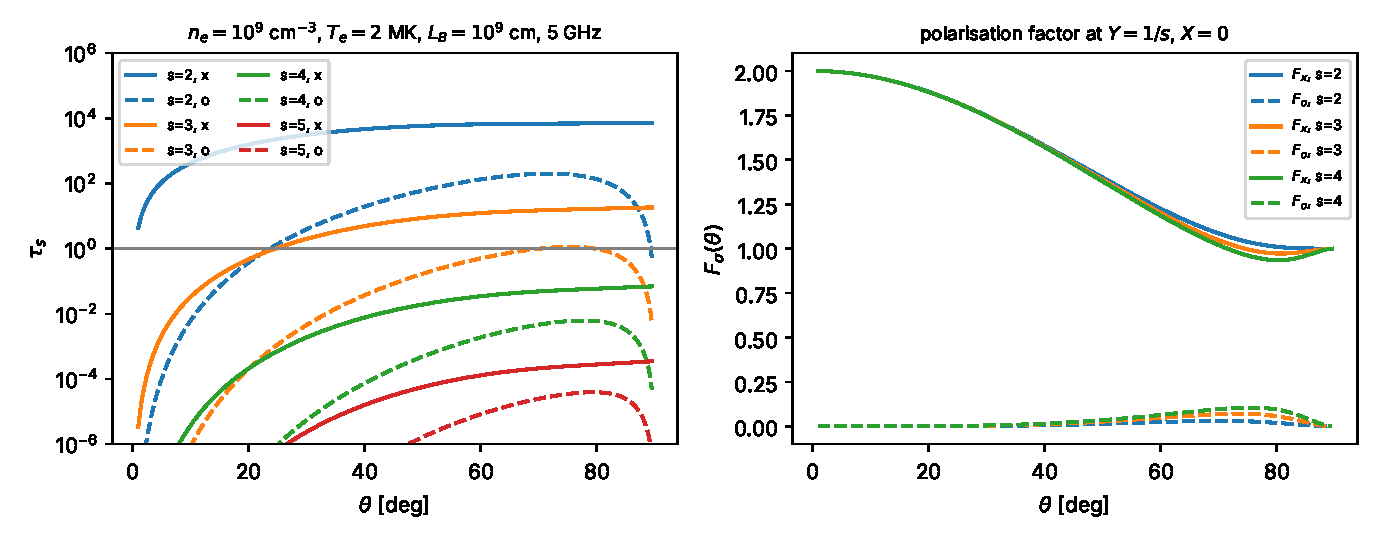
\includegraphics[width=\textwidth]{tau_theta.pdf}
\caption{Left: layer optical depth, Eq.~\eqref{eq:tau}, against the angle between $\vect B$
and the line of sight for $s=2$--5 (solid: x-mode, dashed: o-mode), with the parameters of
Table~\ref{tab:tau}. Right: the polarisation factor $F_\sigma(\theta)$, Eq.~\eqref{eq:F},
on the layers $s=2$, 3, 4 ($X=0$). Both panels were computed with the functions of
\code{gyroresonance/opacity.py}.}
\label{fig:tau}
\end{figure}

\begin{incode}
\code{gyroresonance/opacity.py}: \code{mode\_factor(X, Y, cos, mode)} returns $F_\sigma$
(Eq.~\ref{eq:F}) with $|T_x|$ from \code{axial\_ratio\_x} at $Y=1/s$;
\code{layer\_optical\_depth(s, ne, te, cos, l\_b, freq, mode, X)} returns
Eq.~\eqref{eq:tau} with $\beta_T^2=\kB T_e/(m_ec^2)$ and $\sin^2\theta=\max(1-\cos^2\theta,0)$;
\code{harmonic\_field(s, freq)} returns $B_s$.
\end{incode}

%======================================================================
\section{Kirchhoff's law and the source function}\label{sec:kirchhoff}
%======================================================================

For a thermal plasma Kirchhoff's law holds for each mode separately. With $n_\sigma=1$ each
mode carries half of the Rayleigh--Jeans intensity, so the source function of mode $\sigma$ is
\begin{equation}
  S_\sigma=\frac{\nu^2\kB T_e}{c^2}=\frac12B_\nu^\text{RJ}(T_e).
  \label{eq:source}
\end{equation}
An optically thick layer therefore has brightness temperature $T_e$ \emph{in that mode}, and an
optically thick isothermal source that is thick in both modes is unpolarised.

\begin{incode}
\code{gyroresonance/transfer.py}: the constant \code{\_SRC} $=\kB/c^2$, so that
$S=\code{\_SRC}\,\nu^2T$; \code{bremsstrahlung/magnetized.py}: \code{rayleigh\_jeans\_mode}.
\end{incode}

%======================================================================
\section{Magnetised free--free absorption}\label{sec:ff}
%======================================================================

\subsection{Unmagnetised coefficient}
The thermal free--free (bremsstrahlung) absorption coefficient is, in the default of the
gyroresonance images, the Coulomb-logarithm form of Dulk (1985, Eq.~21),
\begin{equation}
  \kappa_\text{ff}=9.78\times10^{-3}\,\frac{n_e^2}{\nu^2T_e^{3/2}}\,G
  \quad[\text{cm}^{-1},\ n_e\text{ in cm}^{-3}],
  \label{eq:dulk}
\end{equation}
\begin{equation}
  G=\begin{cases}
     18.2+\ln T_e^{3/2}-\ln\nu, & T_e<2\times10^5\,\text{K},\\
     24.5+\ln T_e-\ln\nu, & T_e\ge2\times10^5\,\text{K},
    \end{cases}
\end{equation}
with $G\ge1$, converted to m$^{-1}$. Alternatively (\code{gaunt}$=g$, a number) the code uses
the expression of Moschou et al.\ (2018) with a constant Gaunt factor,
\begin{equation}
  \kappa_\text{ff}=\frac43\sqrt{\frac{2\pi}{3}}\left[\frac{e^2/4\pi\varepsilon_0}{\sqrt{\kB T_e\,m_e}}\right]^3
  \left(\frac{n_e}{\nu}\right)^2\frac{g}{c}.
\end{equation}
Both use the total source function $B_\nu^\text{RJ}=2\nu^2\kB T_e/c^2$. For the parameters of
Table~\ref{tab:tau}, $\kappa_\text{ff}=2.3\times10^{-10}$\,m$^{-1}$ (Dulk) or
$2.5\times10^{-10}$\,m$^{-1}$ ($g=10$): over $10^9$\,cm the corona is thin in free--free at 5\,GHz,
while the $s=2$ and 3 layers are thick.

\subsection{The two modes}
In a magnetic field the free--free absorption differs between the modes. For $Y<1$ and away
from quasi-transverse propagation (Zheleznyakov 1970; Dulk 1985; Gelfreikh 2004),
\begin{equation}
  \kappa_\sigma=\frac{\kappa_\text{ff}}{\left(1+\sigma q\right)^2},\qquad
  q=\min\!\left(Y|\cos\theta|,\ 0.9\right),\qquad
  \sigma=+1\ (\text{o}),\ -1\ (\text{x}),
  \label{eq:ffmode}
\end{equation}
with $S_\sigma$ from Eq.~\eqref{eq:source} for each mode, so that the two modes together give
$B_\nu^\text{RJ}$ in the thick limit. The cap $q\le0.9$ avoids the divergence of the
approximation near the fundamental layer ($Y\to1$).

For an optically thin source the degree of circular polarisation is
\begin{equation}
  \frac{|V|}{I}=\frac{\kappa_x-\kappa_o}{\kappa_x+\kappa_o}
  =\frac{(1+q)^2-(1-q)^2}{(1+q)^2+(1-q)^2}=\frac{2q}{1+q^2}\simeq2Y|\cos\theta|,
  \label{eq:ffpol}
\end{equation}
in the sense of the x-mode; for a thick isothermal source $V\to0$.

\begin{incode}
\code{bremsstrahlung/emission.py}: \code{bremsstrahlung\_coefficients} (Eq.~\ref{eq:dulk} or
the constant-$g$ form; $T_e$ is floored at 1\,K); \code{bremsstrahlung/magnetized.py}:
\code{magnetized\_ff\_coefficients} returns $(\kappa_o,\kappa_x,S_\sigma)$ of
Eq.~\eqref{eq:ffmode} (\code{y\_max}$=0.9$). Keyword \code{gaunt} of \code{make\_gr\_image}
(default \code{"dulk"}).
\end{incode}

%======================================================================
\section{Discretisation: steps and layers}\label{sec:layers}
%======================================================================

\subsection{Free--free part of a step}
The free--free optical depth of step $k$ is evaluated at its mid-point, with the arithmetic
means $\bar q_k=\tfrac12(q_k+q_{k+1})$ of $n_e$, $T_e$, $\cos\theta$ and $B$:
\begin{equation}
  \Delta\tau^\sigma_{\text{ff},k}=\kappa_\sigma\!\left(\bar n_{e,k},\bar T_{e,k},\bar B_k,\overline{\cos\theta}_k\right)\Delta\ell_k .
\end{equation}

\subsection{Finding the layers}
Harmonic $s$ has a layer in step $k$ if $s\nuB-\nu$ changes sign between the nodes,
\begin{equation}
  \left(s\,\nu_{B,k}-\nu\right)\left(s\,\nu_{B,k+1}-\nu\right)<0 .
\end{equation}
The crossing is located by linear interpolation of $\nuB$,
\begin{equation}
  u=\frac{\nu/s-\nu_{B,k}}{\nu_{B,k+1}-\nu_{B,k}}\in(0,1),
\end{equation}
and the plasma parameters on the layer are interpolated with the same weight,
\begin{equation}
  q_c=q_k+u\,(q_{k+1}-q_k)\qquad\text{for } n_e,\ T_e,\ \cos\theta,\ X .
\end{equation}
The magnetic scale length is the finite-difference estimate
\begin{equation}
  L_B=\frac{B_s\,\Delta\ell_k}{|B_{k+1}-B_k|},\qquad B_s=\frac{\nu}{s\,\nuB/\text{G}},
  \label{eq:LB}
\end{equation}
i.e.\ $|B/(\dd B/\dd\ell)|$ on the layer. With these values Eq.~\eqref{eq:tau} gives
$\tau^x_{s,k}$ and $\tau^o_{s,k}$. On the fundamental layer the x-mode is cut off for any
$X>0$ (Eq.~\ref{eq:cutoff} with $Y=1$), so
\begin{equation}
  \tau^x_{1,k}=0\quad\text{if } X_c>0 .
\end{equation}
All harmonics $1\le s\le s_\text{max}$ are tested in every step; several layers can fall into
the same step. Because the layers are thinner than a step, treating each of them as a
discontinuity of optical depth is exact as long as $\Delta s$ resolves $L_B$; one harmonic
crossed twice within one step (if $B$ is not monotonic within it) would be missed, which is a
further reason to keep $\Delta s$ below the scale of the field.

\subsection{Total optical depth and source function of a step}
For each mode the step has
\begin{equation}
  \Delta\tau^\sigma_k=\Delta\tau^\sigma_{\text{ff},k}+\sum_{s}\tau^\sigma_{s,k},
  \qquad
  W^\sigma_k=\Delta\tau^\sigma_{\text{ff},k}\,\bar T_{e,k}+\sum_s\tau^\sigma_{s,k}\,T_{e,c},
\end{equation}
and its source function is the optical-depth-weighted mean
\begin{equation}
  S^\sigma_k=\frac{\nu^2\kB}{c^2}\,\frac{W^\sigma_k}{\Delta\tau^\sigma_k}
  \qquad(0\text{ if }\Delta\tau^\sigma_k=0).
  \label{eq:Seff}
\end{equation}
This is exact for an isothermal step and keeps Kirchhoff's law: a step that is thick only in
one of its layers emits at the temperature of that layer.

\begin{incode}
\code{gyroresonance/transfer.py}, function \code{transfer\_chunk}: mid-step means (\code{m(...)}),
\code{dtau\_o}, \code{dtau\_x}; the loop \code{for s in range(1, s\_max + 1)} with the test
\code{cross}, the weight \code{u}, \code{lerp}, \code{l\_b} (Eq.~\ref{eq:LB}),
\code{layer\_optical\_depth} for both modes and the $s=1$ rule; the sums \code{gr\_x},
\code{gr\_o} ($\sum_s\tau_s$) and \code{st\_x}, \code{st\_o} ($W$). Keyword \code{s\_max};
\code{mechanisms="gr"} or \code{"ff"} keeps only one of the two parts.
\end{incode}

%======================================================================
\section{Radiative transfer along the line of sight}\label{sec:transfer}
%======================================================================

For each of the two polarisations $p$ (Sect.~\ref{sec:coupling} says which mode coefficients
each one uses in each step) the formal solution of
$\dd I_p/\dd\tau=S_p-I_p$, summed from the observer inwards with $S_p$ constant within a step,
is
\begin{equation}
  \boxed{\;
  I_p=\sum_{k=0}^{N-1}S^p_k\left(1-e^{-\Delta\tau^p_k}\right)\exp\!\Big(-\sum_{j<k}\Delta\tau^p_j\Big)
  \;+\;\frac{\nu^2\kB}{c^2}\,T_\text{body}\,e^{-\tau_p}\,\chi_\text{body}\;}
  \label{eq:transfer}
\end{equation}
where $\tau_p=\sum_k\Delta\tau^p_k$ is the total optical depth of the line, and the last term
(optional) is the emission of the body, with brightness temperature $T_\text{body}$, seen by
lines that end on $r=r_\text{body}$ ($\chi_\text{body}=1$) and are not cut off.

\paragraph{Cutoffs.} A polarisation cannot reach the observer from behind a point where its
mode does not propagate. If node $k$ is a cutoff node for polarisation $p$
(Eq.~\ref{eq:cutoff} evaluated with $X_k$, $Y_k$), the steps from $k$ onwards contribute
nothing:
\begin{equation}
  a^p_k=\prod_{j\le k}\left(1-c^p_j\right),\qquad
  \Delta\tau^p_k\to a^p_{k+1}\,\Delta\tau^p_k,\quad W^p_k\to a^p_{k+1}\,W^p_k,
\end{equation}
where $c^p_j=1$ at a cutoff node inside the domain and 0 otherwise. Lines that are cut off
are flagged (\code{cutoff}).

\begin{incode}
\code{transfer\_chunk}: \code{alive = cumprod(\textasciitilde(c \& live))} ($a^p_k$),
\code{tau\_front = cumsum(d) - d}, \code{S = sw/d * \_SRC * freq**2} (Eq.~\ref{eq:Seff}),
\code{w = exp(-tau\_front) * -expm1(-d)}, \code{I = (S*w).sum(axis=1)}
(Eq.~\ref{eq:transfer}); body term with keyword \code{t\_body} of \code{make\_gr\_image}
(default: no body emission).
\end{incode}

%======================================================================
\section{Mode coupling and the two polarisations}\label{sec:coupling}
%======================================================================

Along a line of sight $\vect B\cdot\hat{\vect k}$ may change sign (a quasi-transverse region,
for instance above the neutral line between two spots). There, the radiation either keeps
its mode identity, so that its sense of circular polarisation reverses (\emph{strong
coupling}, at low frequencies and strong fields), or keeps its sense of polarisation and
changes mode (\emph{weak coupling}, the usual case at microwave frequencies; Cohen 1960).
\textsf{radiosynth} offers both limits.

\paragraph{Weak coupling} (\code{coupling="weak"}, default). The transfer is done for
right- and left-hand circular polarisation, $p\in\{R,L\}$. In each step
\begin{equation}
  (\Delta\tau^R_k,W^R_k)=\begin{cases}(\Delta\tau^x_k,W^x_k), & \overline{\cos\theta}_k>0,\\
                                       (\Delta\tau^o_k,W^o_k), & \overline{\cos\theta}_k\le0,\end{cases}
  \qquad
  (\Delta\tau^L_k,W^L_k)=\text{the other mode},
\end{equation}
and the cutoff of node $k$ is that of the x-mode for $R$ when $\cos\theta_k>0$ (and of the
o-mode otherwise), and conversely for $L$. Then
\begin{equation}
  I=I_R+I_L,\qquad V=I_R-I_L .
\end{equation}

\paragraph{Strong coupling} (\code{coupling="strong"}). The transfer is done for the modes,
$p\in\{x,o\}$, with their own coefficients and cutoffs everywhere, and the sign of $V$ is
set by the field direction at the observer's end of the line (the first node with $B>0$):
\begin{equation}
  I=I_x+I_o,\qquad V=\operatorname{sgn}\!\left(\cos\theta_{k_1}\right)\left(I_x-I_o\right).
\end{equation}
Without a quasi-transverse region the two options give the same result.

\begin{incode}
\code{transfer\_chunk}: the \code{if coupling == "weak"} branch (\code{pos = cos\_m > 0} for
the steps, \code{posn = cos > 0} for the cutoffs) and the \code{"strong"} branch
(\code{vsign}). Keyword \code{coupling} of \code{make\_gr\_image}.
\end{incode}

%======================================================================
\section{Brightness temperature, polarisation and flux}\label{sec:output}
%======================================================================

The image holds, for every frequency and pixel, $I$ and $V$ in
W\,m$^{-2}$\,Hz$^{-1}$\,sr$^{-1}$, and the two polarisations $I_1$, $I_2$ ($R$, $L$ or $x$, $o$).
The Rayleigh--Jeans brightness temperatures are
\begin{equation}
  T_b=\frac{c^2}{2\kB\nu^2}\,I,\qquad
  T_b(V)=\frac{c^2}{2\kB\nu^2}\,V,\qquad
  T_p=\frac{c^2}{\kB\nu^2}\,I_p\quad(p=1,2),
\end{equation}
so that $T_b=\tfrac12(T_1+T_2)$ and $T_p=T_e$ for a polarisation that is optically thick in
isothermal plasma. The degree of circular polarisation is $V/I$ (undefined where $I=0$).
For a pixel of size $\Delta X\Delta Y$ in the image plane at distance $D$ from the observer,
the solid angle is $\Delta\Omega=\Delta X\Delta Y/D^2$ (all in the same unit), and the flux
densities are
\begin{equation}
  F_I=\sum_\text{pixels}I\,\Delta\Omega,\qquad F_V=\sum_\text{pixels}V\,\Delta\Omega,
\end{equation}
in W\,m$^{-2}$\,Hz$^{-1}$ (1\,sfu $=10^{-22}$\,W\,m$^{-2}$\,Hz$^{-1}$).

\begin{incode}
\code{gyroresonance/image.py}, class \code{GRImage}: \code{intensity}, \code{stokes\_v},
\code{pol1}, \code{pol2}, \code{brightness\_temperature}, \code{tb\_v}, \code{tb\_pol},
\code{polarization}, \code{flux\_density}, \code{flux\_density\_v}.
\end{incode}

%======================================================================
\section{Diagnostics}\label{sec:diag}
%======================================================================

The contribution of step $k$ to the observed intensity of polarisation $p$ is
\begin{equation}
  C^p_k=S^p_k\left(1-e^{-\Delta\tau^p_k}\right)\exp\!\Big(-\sum_{j<k}\Delta\tau^p_j\Big).
\end{equation}
It is split between free--free and layers in proportion to their optical depths,
\begin{equation}
  C^{p,\text{GR}}_k=C^p_k\,\frac{\sum_s\tau^p_{s,k}}{\Delta\tau^p_k}.
\end{equation}
From these, for every pixel:
\begin{itemize}
  \item \code{gr\_fraction} $=\sum_{p,k}C^{p,\text{GR}}_k\big/\sum_{p,k}C^p_k$, the share of $I$
        that comes from the layers;
  \item \code{radius} $=\sum_{p,k}C^p_k\,\bar r_k\big/\sum_{p,k}C^p_k$, the intensity-weighted
        radius of the emission ($\bar r_k$: distance of the step's mid-point from the centre);
  \item \code{dominant\_s}: the harmonic whose layers carry most of the intensity (each step's
        layer contribution is attributed to the harmonic with the largest $\tau$ in that step),
        0 if free--free dominates, $-1$ if there is no emission;
  \item \code{x\_flag}: true if a significant layer ($\max(\tau^x,\tau^o)>0.1$) has
        $X>0.25$, where the approximation $n_\sigma=1$ in Eq.~\eqref{eq:tau} becomes rough;
  \item \code{cutoff}: true if a polarisation was stopped at a cutoff.
\end{itemize}

%======================================================================
\section{Assumptions and range of validity}\label{sec:limits}
%======================================================================

\begin{enumerate}
  \item \textbf{Maxwellian electrons, lowest order in $\beta_T$.} Eq.~\eqref{eq:tau} is the
        small-Larmor-radius limit; the relative error is $O(s^2\beta_T^2)$, about 1\,\% or
        less for $s\le6$ at coronal temperatures (0.8\,\% in the test of Sect.~\ref{sec:validation}). Non-thermal electrons are treated by the
        gyrosynchrotron part of \textsf{radiosynth}.
  \item \textbf{Refractive index 1.} Valid for $X\ll1$, normally true where gyroresonance
        emission forms; layers with $X>0.25$ are flagged.
  \item \textbf{o-mode near $\theta=90^\circ$.} At lowest order $F_o\to0$ across the field;
        the true o-mode opacity is then of higher order in $\beta_T$ and is underestimated.
  \item \textbf{Straight lines of sight.} Refraction is neglected (it matters only near the
        plasma level, $X\to1$, where gyroresonance emission does not form).
  \item \textbf{Mode coupling} is treated in the two limits, weak or strong, not with the
        intermediate coupling coefficient.
  \item \textbf{Magnetised free--free} uses Eq.~\eqref{eq:ffmode}, valid for $Y<1$ away from
        quasi-transverse propagation; $Y|\cos\theta|$ is capped at 0.9.
  \item \textbf{Resolution.} The model must resolve $L_B$ and the variation of $n_e$ and
        $T_e$; the step $\Delta s$ must be small enough that each harmonic is crossed at most
        once per step.
  \item \textbf{Chromosphere.} Lines that reach $r_\text{body}$ see nothing behind it unless
        a body temperature $T_\text{body}$ is given.
\end{enumerate}

%======================================================================
\section{Validation}\label{sec:validation}
%======================================================================

The test script \code{tests/test\_gyroresonance.py} checks the implementation against
independent results:
\begin{center}
\small
\begin{tabular}{@{}p{10.5cm} l@{}}
\toprule
Test & Result \\
\midrule
Layer $\tau_s$ vs.\ Maxwellian average of the exact $J_{s-1}^2$ ($s=2$--6) & $\le0.8\,\%$ ($=O(s^2\beta_T^2)$) \\
Single $s=3$ layer in a linear field: $I=S(1-e^{-\tau})$ per mode & $10^{-6}$ \\
Thick layers: $T_b(R)=T_b(L)=T_e$ & $2\times10^{-11}$ \\
$V$ sign over the positive spot; $\vect B\to-\vect B$ gives $V\to-V$ & exact \\
Straight-ray free--free vs.\ refractive tracer without refraction & $5\times10^{-4}$ \\
Thin magnetised free--free: $V/I=2q/(1+q^2)$, Eq.~\eqref{eq:ffpol} & $3\times10^{-4}$ \\
Spherical grid $(B_r,B_\theta,B_\phi)$ vs.\ Cartesian image ($I$; $V$) & 0.8\,\%; 1.8\,\% \\
PLUTO \code{bx1..3} in code units $\to$ gauss & $10^{-11}$ \\
\bottomrule
\end{tabular}
\end{center}

%======================================================================
\section{Using it}\label{sec:use}
%======================================================================

\begin{small}
\begin{verbatim}
import radiosynth as rs
grid = rs.load_pluto("out/", with_b=True)     # or rs.load_mhd(..., with_b=True)
img = rs.make_gr_image(grid, "3GHz, 5GHz, 17GHz", observer=(-215, 0, 0),
                       x_size=0.4, y_size=0.4, nx=200, ny=200,
                       mechanisms="gr+ff", gaunt="dulk", s_max=10, coupling="weak")
img.plot("tb"); img.plot("pol"); img.plot("harmonic")
print(img.summary())
\end{verbatim}
\end{small}
or, from the command line,
\begin{small}
\begin{verbatim}
python -m radiosynth ar.dat --mechanism gyroresonance --freq "5GHz, 17GHz" \
       --size 0.4 0.4 --npix 200 200 --out gr --plot
\end{verbatim}
\end{small}

\begin{center}
\small
\begin{tabular}{@{}l l@{}}
\toprule
Keyword of \code{make\_gr\_image} & Quantity in this note \\
\midrule
\code{mechanisms} (\code{"gr+ff"}, \code{"gr"}, \code{"ff"}) & which of $\tau_s^\sigma$, $\Delta\tau_\text{ff}^\sigma$ are included \\
\code{gaunt} (\code{"dulk"} or a number) & $\kappa_\text{ff}$, Sect.~\ref{sec:ff} \\
\code{s\_max} & highest harmonic $s$ \\
\code{coupling} (\code{"weak"}, \code{"strong"}) & Sect.~\ref{sec:coupling} \\
\code{ds} & step $\Delta s$ [coordinate units] \\
\code{t\_body} & $T_\text{body}$ in Eq.~\eqref{eq:transfer} \\
\code{observer}, \code{distance\_pc}, \code{x\_size}, \code{nx}, \ldots & geometry, Sect.~\ref{sec:geometry} \\
\bottomrule
\end{tabular}
\end{center}

%======================================================================
\section*{References}
\addcontentsline{toc}{section}{References}
%======================================================================
\begin{small}
\begin{itemize}[leftmargin=1.2em,itemsep=1pt]
\item Cohen, M.\ H.\ 1960, ApJ 131, 664 --- mode coupling in quasi-transverse regions.
\item Dulk, G.\ A.\ 1985, ARA\&A 23, 169 --- radio emission from the Sun and stars.
\item Fleishman, G.\ D., \& Kuznetsov, A.\ A.\ 2014, ApJ 781, 77 --- gyroresonance and free--free
      emission from non-Maxwellian distributions.
\item Gelfreikh, G.\ B.\ 2004, in \emph{Solar and Space Weather Radiophysics}, ASSL 314, 115 ---
      polarisation of thermal free--free emission.
\item Melrose, D.\ B.\ 1980, \emph{Plasma Astrophysics} (Gordon \& Breach).
\item Moschou, S.-P., Sokolov, I., Cohen, O., et al.\ 2018, ApJ 867, 51.
\item White, S.\ M., \& Kundu, M.\ R.\ 1997, Sol.\ Phys.\ 174, 31 --- gyroresonance emission from
      coronal magnetic fields.
\item Zheleznyakov, V.\ V.\ 1970, \emph{Radio Emission of the Sun and Planets} (Pergamon).
\end{itemize}
\end{small}

\end{document}
